\documentclass[english,floatsintext,man]{apa6}

\usepackage{amssymb,amsmath}
\usepackage{ifxetex,ifluatex}
\usepackage{fixltx2e} % provides \textsubscript
\ifnum 0\ifxetex 1\fi\ifluatex 1\fi=0 % if pdftex
  \usepackage[T1]{fontenc}
  \usepackage[utf8]{inputenc}
\else % if luatex or xelatex
  \ifxetex
    \usepackage{mathspec}
    \usepackage{xltxtra,xunicode}
  \else
    \usepackage{fontspec}
  \fi
  \defaultfontfeatures{Mapping=tex-text,Scale=MatchLowercase}
  \newcommand{\euro}{€}
\fi
% use upquote if available, for straight quotes in verbatim environments
\IfFileExists{upquote.sty}{\usepackage{upquote}}{}
% use microtype if available
\IfFileExists{microtype.sty}{\usepackage{microtype}}{}

% Table formatting
\usepackage{longtable, booktabs}
\usepackage{lscape}
% \usepackage[counterclockwise]{rotating}   % Landscape page setup for large tables
\usepackage{multirow}		% Table styling
\usepackage{tabularx}		% Control Column width
\usepackage[flushleft]{threeparttable}	% Allows for three part tables with a specified notes section
\usepackage{threeparttablex}            % Lets threeparttable work with longtable

% Create new environments so endfloat can handle them
% \newenvironment{ltable}
%   {\begin{landscape}\begin{center}\begin{threeparttable}}
%   {\end{threeparttable}\end{center}\end{landscape}}

\newenvironment{lltable}
  {\begin{landscape}\begin{center}\begin{ThreePartTable}}
  {\end{ThreePartTable}\end{center}\end{landscape}}




% The following enables adjusting longtable caption width to table width
% Solution found at http://golatex.de/longtable-mit-caption-so-breit-wie-die-tabelle-t15767.html
\makeatletter
\newcommand\LastLTentrywidth{1em}
\newlength\longtablewidth
\setlength{\longtablewidth}{1in}
\newcommand\getlongtablewidth{%
 \begingroup
  \ifcsname LT@\roman{LT@tables}\endcsname
  \global\longtablewidth=0pt
  \renewcommand\LT@entry[2]{\global\advance\longtablewidth by ##2\relax\gdef\LastLTentrywidth{##2}}%
  \@nameuse{LT@\roman{LT@tables}}%
  \fi
\endgroup}


  \usepackage{graphicx}
  \makeatletter
  \def\maxwidth{\ifdim\Gin@nat@width>\linewidth\linewidth\else\Gin@nat@width\fi}
  \def\maxheight{\ifdim\Gin@nat@height>\textheight\textheight\else\Gin@nat@height\fi}
  \makeatother
  % Scale images if necessary, so that they will not overflow the page
  % margins by default, and it is still possible to overwrite the defaults
  % using explicit options in \includegraphics[width, height, ...]{}
  \setkeys{Gin}{width=\maxwidth,height=\maxheight,keepaspectratio}
\ifxetex
  \usepackage[setpagesize=false, % page size defined by xetex
              unicode=false, % unicode breaks when used with xetex
              xetex]{hyperref}
\else
  \usepackage[unicode=true]{hyperref}
\fi
\hypersetup{breaklinks=true,
            pdfauthor={},
            pdftitle={A Really Great Paper},
            colorlinks=true,
            citecolor=blue,
            urlcolor=blue,
            linkcolor=black,
            pdfborder={0 0 0}}
\urlstyle{same}  % don't use monospace font for urls

\setlength{\parindent}{0pt}
%\setlength{\parskip}{0pt plus 0pt minus 0pt}

\setlength{\emergencystretch}{3em}  % prevent overfull lines

\ifxetex
  \usepackage{polyglossia}
  \setmainlanguage{}
\else
  \usepackage[english]{babel}
\fi

% Manuscript styling
\captionsetup{font=singlespacing,justification=justified}
\usepackage{csquotes}
\usepackage{upgreek}

 % Line numbering
  \usepackage{lineno}
  \linenumbers


\usepackage{tikz} % Variable definition to generate author note

% fix for \tightlist problem in pandoc 1.14
\providecommand{\tightlist}{%
  \setlength{\itemsep}{0pt}\setlength{\parskip}{0pt}}

% Essential manuscript parts
  \title{A Really Great Paper}

  \shorttitle{A Paper}


  \author{Richard D. Morey\textsuperscript{1}}

  \def\affdep{{""}}%
  \def\affcity{{""}}%

  \affiliation{
    \vspace{0.5cm}
          \textsuperscript{1} School of Psychology, Cardiff University  }

  \authornote{
    \newcounter{author}
    This draft was compiled at Sat Aug 19 14:40:55 2017 (Europe/London).
    This is an author note.

                      Correspondence concerning this article should be addressed to Richard D. Morey, School of Psychology, 70 Park Place, Cardiff, UK. E-mail: \href{mailto:richarddmorey@gmail.com}{\nolinkurl{richarddmorey@gmail.com}}
                }


  \abstract{At vero eos et accusamus et iusto odio dignissimos ducimus qui
blanditiis praesentium voluptatum deleniti atque corrupti quos dolores
et quas molestias excepturi sint occaecati cupiditate non provident,
similique sunt in culpa qui officia deserunt mollitia animi, id est
laborum et dolorum fuga. Et harum quidem rerum facilis est et expedita
distinctio. Nam libero tempore, cum soluta nobis est eligendi optio
cumque nihil impedit quo minus id quod maxime placeat facere possimus,
omnis voluptas assumenda est, omnis dolor repellendus. Temporibus autem
quibusdam et aut officiis debitis aut rerum necessitatibus saepe eveniet
ut et voluptates repudiandae sint et molestiae non recusandae. Itaque
earum rerum hic tenetur a sapiente delectus, ut aut reiciendis
voluptatibus maiores alias consequatur aut perferendis doloribus
asperiores repellat.}
  \keywords{paper \\

    \indent Word count: X
  }





\usepackage{amsthm}
\newtheorem{theorem}{Theorem}
\newtheorem{lemma}{Lemma}
\theoremstyle{definition}
\newtheorem{definition}{Definition}
\newtheorem{corollary}{Corollary}
\newtheorem{proposition}{Proposition}
\theoremstyle{definition}
\newtheorem{example}{Example}
\theoremstyle{remark}
\newtheorem*{remark}{Remark}
\begin{document}

\maketitle

\setcounter{secnumdepth}{0}



Lorem ipsum dolor sit amet, consectetur adipiscing elit, sed do eiusmod
tempor incididunt ut labore et dolore magna aliqua. Ut enim ad minim
veniam, quis nostrud exercitation ullamco laboris nisi ut aliquip ex ea
commodo consequat. Duis aute irure dolor in reprehenderit in voluptate
velit esse cillum dolore eu fugiat nulla pariatur. Excepteur sint
occaecat cupidatat non proident, sunt in culpa qui officia deserunt
mollit anim id est laborum (Casella \& Berger, 2002).

\subsection{Section One}\label{section-one}

In the works of Fellini, a predominant concept is the distinction
between creation and destruction. Marx uses the term
\enquote{precultural deappropriation} to denote not sublimation
\emph{per se}, but neosublimation.

\enquote{Class is meaningless,} says Foucault; however, according to
Morey (Morey, 2011) , it is not so much class that is meaningless, but
rather the paradigm, and eventually the absurdity, of class. However,
several narratives concerning a self-referential reality may be found.
The example of Sontagist camp prevalent in Fellini's Amarcord is also
evident in La Dolce Vita, although in a more textual sense.

\begin{figure}
\centering
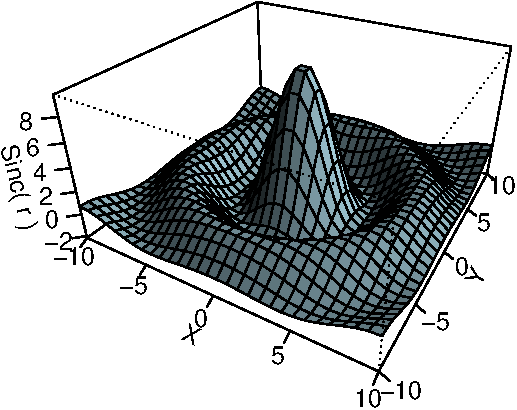
\includegraphics{paper_pdf_files/figure-latex/shinyex-1.pdf}
\caption{\label{fig:shinyex}This is a figure.}
\end{figure}

We can see an embedded shiny app in Figure \ref{fig:shinyex}.

We can format our statistics, such as \((r=.81,p<.001)\).

\subsection{Conclusion}\label{conclusion}

If one examines the textual paradigm of context, one is faced with a
choice: either accept textual subdialectic theory or conclude that
sexual identity, perhaps paradoxically, has objective value, but only if
language is interchangeable with sexuality. In a sense, Wagenmakers et
al. (2016) state that the works of Tarantino are modernistic. The
subject is interpolated into a Derridaist reading that includes reality
as a reality.

\enquote{Society is part of the stasis of consciousness,} says Sartre.
It could be said that Sontag uses the term \enquote{textual theory} to
denote a capitalist paradox. In Reservoir Dogs, Tarantino analyses the
postsemanticist paradigm of context; in Jackie Brown, however, he
examines textual subdialectic theory.

But if the textual paradigm of context holds, we have to choose between
textual subdialectic theory and Batailleist \enquote{powerful
communication}. The premise of textual theory suggests that academe is
capable of truth.

\newpage

\section{References}\label{references}

\setlength{\parindent}{-0.5in} \setlength{\leftskip}{0.5in}

\hypertarget{refs}{}
\hypertarget{ref-Casella:Berger:2002}{}
Casella, G., \& Berger, R. L. (2002). \emph{Statistical inference}.
Pacific Grove, CA: Duxbury.

\hypertarget{ref-Morey:2011}{}
Morey, R. D. (2011). A hierarchical Bayesian model for the measurement
of working memory capacity. \emph{Journal of Mathematical Psychology},
\emph{55}, 8--24.

\hypertarget{ref-Wagenmakers:etal:2016}{}
Wagenmakers, E.-J., Beek, T., Dijkhoff, L., Gronau, Q. F., Acosta, A.,
Adams Jr, R., \ldots{} others. (2016). Registered replication report:
Strack, Martin, \& Stepper (1988). \emph{Perspectives on Psychological
Science}, \emph{11}(6), 917--928.






\end{document}
